% MLSA 2026 submission
% Springer LNCS, 9 content pages + unlimited references
% Submission deadline: 5 June 2026, 23:59 AoE
% Camera-ready: 10 July 2026
% Workshop: 7 September 2026, Naples, Italy
% Submission via CMT; in-person presentation required.

\documentclass[runningheads,a4paper]{llncs}

\usepackage[T1]{fontenc}
\usepackage[utf8]{inputenc}
\usepackage{graphicx}
\usepackage{amsmath}
\usepackage{amssymb}
\usepackage{booktabs}
\usepackage{makecell}
\usepackage{microtype}
\usepackage[hidelinks,
            pdftitle={Spatial Resolution and Token Count Matter:
                      A CNN+Transformer Hybrid for Image-Based Expected Goals},
            pdfauthor={Mustafa Burkay Ozdemir and Nejat Yumusak}]{hyperref}
\usepackage{cite}

\title{Spatial Resolution and Token Count Matter:\texorpdfstring{\\}{ }%
A CNN+Transformer Hybrid for Image-Based Expected Goals}

\titlerunning{Image-Based xG with CNN+Transformer Hybrids}

\author{Mustafa Burkay \"Ozdemir\inst{1}\orcidID{0009-0007-3701-0084} \and
Nejat Yumu\c{s}ak\inst{1}\orcidID{0000-0001-5005-8604}}

\authorrunning{M. B. \"Ozdemir and N. Yumu\c{s}ak}

\institute{Sakarya University, Department of Computer Engineering, Sakarya, Turkey\\
\email{mustafa.ozdemir24@ogr.sakarya.edu.tr, nyumusak@sakarya.edu.tr}}

\begin{document}

\maketitle

% ============================================================
% ABSTRACT — target 200 words
% Source: CLAIMS.md Section 1 (Headline claims C1–C7)
% ============================================================
\begin{abstract}
Image-based Expected Goals (xG) renders the StatsBomb shot freeze
frame as a top-down image and lets a vision model read spatial
context. To our knowledge, prior image-based xG work has used
CNN-style architectures. We add a CNN+Transformer hybrid and ask
under what conditions attention helps.
Under a strictly controlled rendering protocol (sigma specified in
pitch-coordinate units, penalty-excluded, four channels: attackers,
defenders, goalkeeper, shooter), a Hybrid CNN+Transformer at
$128{\times}128$ outperforms the $64{\times}64$ CNN baseline on every
headline metric across three training seeds: ROC-AUC $+0.003$,
PR-AUC $+0.014$, F1 $+0.006$, Platt Brier $-0.001$. The lift grows
with transformer token count, and pure-CNN PR-AUC degrades
monotonically with resolution while the hybrid recovers at 64 tokens.
A $2{\times}2$ $\sigma{\times}$\,penalty ablation shows that penalty
inclusion has near-zero main effect on PR-AUC and a strong
$\sigma$-conditional interaction; the apparent penalty bias seen in
cross-protocol comparisons is therefore not a single-variable effect.
We release a PyTorch reference implementation with explicit
pitch-unit sigma.

\keywords{Expected Goals \and Football Analytics \and CNN \and Transformer
\and Image-Based xG \and StatsBomb.}
\end{abstract}

% ============================================================
% 1. INTRODUCTION  (target: ~1 page)
% Source: PAPER_OUTLINE.md Section 2 (Motivation, Gap, Contributions, Negative findings)
% ============================================================
\section{Introduction}
\label{sec:intro}

Expected Goals (xG) is the per-shot probability of scoring and the
most widely used probabilistic shot-quality metric in football
analytics. Tabular xG models with hand-engineered features (shot
location, body part, assist type, play pattern) dominate practice and
reach validation AUC in the $0.80$--$0.88$
range~\cite{anzer2021xg}, but they cannot read the spatial context
around the shooter: defender pressure, keeper position, and the
geometry of the goal mouth at the moment of the shot. Image-based xG
addresses this gap by rendering the StatsBomb shot freeze-frame as a
top-down image and letting a vision model learn from spatial layout
directly~\cite{wagenaar2017xg,matteotti2024xgcnn}.

Vision Transformers and CNN+Transformer hybrids dominate generic image
recognition~\cite{vaswani2017attention,dosovitskiy2021vit}, yet to our
knowledge prior image-based xG work has used CNN-style architectures.
The most recent end-to-end image-based xG,
xG-CNN~\cite{matteotti2024xgcnn}, is a two-channel CNN (opponent
locations and ball position) on a $30{\times}40$ offensive-half grid
and reports validation AUC $\approx 0.80$ with no attention.
Skor-xG~\cite{xu2025skorxg} uses graph attention on 3D skeletons, a
different modality. No published image-based xG study isolates the
effects of (i) input resolution, (ii) Gaussian rendering sigma, and
(iii) self-attention on the freeze-frame representation.

\paragraph{Contributions.}
\begin{enumerate}\itemsep0pt
  \item A controlled six-cell ablation (CNN/Hybrid $\times$ 64/96/128) at
        fixed $\sigma_{\text{pu}}=2.0$ with penalties excluded,
        three seeds per cell.
  \item A token-count sweep showing that the hybrid's lift over the
        CNN at fixed sigma correlates with the transformer's effective
        token count (16 $\rightarrow$ 36 $\rightarrow$ 64).
  \item A five-point sigma sweep at $128{\times}128$ showing that
        pixel-fixed sigma is a hidden hyperparameter and that the
        resolution-appropriate sigma is $\approx 2$ pitch units,
        much smaller than the 64-pixel baseline's pitch-equivalent.
  \item A $2{\times}2$ ($\sigma{\times}$\,penalty) ablation at
        $64{\times}64$ isolating that penalty inclusion does
        \emph{not} bias PR-AUC upward by itself (main effect
        $\approx 0$); the effect is $\sigma$-conditional.
  \item A reproducible PyTorch reference implementation with explicit
        pitch-unit sigma specification.
\end{enumerate}

\paragraph{Positioning vs.\ xG-CNN.}
We extend the image-based xG framework with a four-channel full-pitch
representation, explicit pitch-unit sigma, and a CNN+Transformer
hybrid. A direct numeric comparison with xG-CNN's reported
AUC~$\approx 0.80$ is not strictly valid here: the two pipelines
differ on channel structure, pitch coverage, grid, dataset filter,
class weighting, and validation protocol. We therefore treat xG-CNN
as methodological motivation rather than a numeric baseline; a strict
replication under our protocol is future work. Related work that
applies attention to football data~\cite{xu2025skorxg,fernandez2021epv}
operates on 3D skeletons or tracking streams and does not overlap with
our image-based setting.

% ============================================================
% Related Work folded into Section 1 (Introduction).
% No standalone Related Work section because of the 9-page LNCS budget;
% positioning vs xG-CNN, Skor-xG, Wagenaar 2017, Anzer-Bauer 2021, and
% Fernandez-Bornn-Cervone 2021 will appear as a single paragraph at the
% end of Section 1 ("Positioning") and a short footnote where needed.
% ============================================================

% ============================================================
% 3. METHOD  (target: ~1.5 pages)
% Source: PAPER_OUTLINE.md Section 4 + HYPERPARAMETERS.md
% ============================================================
\section{Method}
\label{sec:method}

\subsection{Data and Splits}
\label{sec:data}

We use StatsBomb open-data~\cite{statsbomb_opendata}, containing 88{,}023
shot events. We discard shots with empty
\texttt{shot\_freeze\_frame} fields (leaving 86{,}833 renderable shots)
and exclude penalty shots (\texttt{shot\_type == ``Penalty''}) for the
controlled headline runs, yielding 86{,}662 shots. The penalty exclusion
is a deliberate design choice: StatsBomb leaves the freeze-frame array
empty for most penalties (1{,}190 of the 1{,}361 raw penalties are
already removed by the freeze-frame check), so the remaining 171 are
structurally different from the open-play distribution. We analyze the
penalty-handling decision empirically in Section~\ref{sec:2x2}.

We split at the match level (70/15/15) with stratification on per-match
goal counts and a fixed random seed of 42. The final controlled splits
are train 60{,}893 / val 12{,}642 / test 13{,}127, with a goal rate of
$\approx 10.15\%$ in all three splits. Match-level splitting prevents
match-level leakage: shots from the same match cannot appear across
splits, so the validation and test sets cannot share the configuration
of a specific game state with the training set.

\subsection{Rendering in Pitch-Coordinate Units}
\label{sec:rendering}

Each shot is rendered as a four-channel top-down image: (i) attackers
(teammates of the shooter excluding the shooter), (ii) defenders,
(iii) goalkeeper, (iv) shooter. Each player contributes an isotropic
Gaussian blob with amplitude 1, clipped to $[0,1]$.

\textbf{Sigma in pitch-coordinate units.}
StatsBomb uses a native $120{\times}80$ pitch-coordinate frame; these
units are \emph{not} literal meters and we do not apply a fixed UEFA
conversion (1\,pu $\approx 0.875$\,m on a $105{\times}68$\,m pitch).
Instead, we specify the Gaussian standard deviation $\sigma_{\text{pu}}$
directly in pitch-coordinate units and convert to pixels at render
time using
$\sigma_{\text{px}} = \sigma_{\text{pu}} \cdot W / 120$,
where $W$ is the image width. This decouples the physical smoothing
from the image resolution: a fixed $\sigma_{\text{px}}$ would scale
the blob's physical area inversely with $W$, which we show in
Section~\ref{sec:sigma-sweep} is a hidden hyperparameter that
materially affects PR-AUC. All controlled headline runs use
$\sigma_{\text{pu}}=2.0$.

\textbf{Attack-direction normalization.}
Half of the shots in StatsBomb attack toward the left goal and half
toward the right. We normalize all shots to attack toward the right
goal by flipping shots in the first group horizontally and mirroring
their $y$-coordinates. The model therefore never sees attack direction
as an input variable, which improves sample efficiency by aligning
mirror-symmetric game situations into a single coordinate frame.

\subsection{Architectures}
\label{sec:arch}

\textbf{CNN-XG.}
Four convolutional blocks with $\{32, 64, 128, 256\}$ output channels.
Each block is two $3{\times}3$ convolutions with batch normalization
and ReLU, followed by $2{\times}2$ max pooling; we apply
\texttt{Dropout2d(0.05)} after the third and fourth blocks.
The conv backbone ends in
\texttt{AdaptiveAvgPool2d((1,1))}, which gives a fixed 256-dimensional
representation independent of the input resolution. The classification
head is \texttt{Linear(256, 128)} + ReLU + \texttt{Dropout(0.3)} +
\texttt{Linear(128, 1)} with a sigmoid output. The model has
$\approx 1.21$\,M parameters at every resolution.

\textbf{Hybrid CNN+Transformer-XG.}
The same conv backbone produces a feature map of size
$(H/16) \times (W/16) \times 256$, which we flatten into a sequence of
$T = (H/16) \cdot (W/16)$ tokens of dimension 256. Token counts are
$T = 16, 36, 64$ at input resolutions $64, 96, 128$ respectively.
A learnable positional embedding is sliced to length $T$ and added to
the tokens. Four transformer encoder layers~\cite{vaswani2017attention}
process the tokens with $8$ attention heads, FFN dimension 512, GELU
activation, and pre-norm; we use the standard
\texttt{nn.TransformerEncoderLayer} implementation. The output is mean
pooled across tokens and passed through the same MLP head as the CNN.
Parameter counts are $\approx 3.32$\,M at $64{\times}64$ and
$\approx 3.33$\,M at $128{\times}128$; the $\approx 12$k difference is
the larger positional embedding ($64 - 16$ extra tokens at dimension
256).

\subsection{Training and Evaluation}
\label{sec:training}

We train with binary cross-entropy on logits and the positive-class
weight set to the train-split imbalance ratio,
$\text{pos\_weight} = N_{\text{neg}} / N_{\text{pos}} \approx 8.85$.
The optimizer is AdamW~\cite{loshchilov2019adamw} with learning rate
$10^{-4}$ and weight decay $10^{-5}$; we reduce the learning rate by
half on validation-loss plateaus with patience 5 and a floor of
$10^{-7}$. Training stops when validation ROC-AUC has not improved for
10 epochs and we restore the best-validation checkpoint. CNN runs are
capped at 15 epochs with batch size 128 at $64{\times}64$ and 64 at
higher resolutions; hybrid runs are capped at 30 epochs with batch size
64 and typically stop by epoch 18--22. All training uses Apple Silicon
MPS without mixed precision and the PyTorch
implementation~\cite{paszke2019pytorch}.

\textbf{Seed repeats.}
The match-level split uses a fixed random seed (42); the training-time
seed we vary controls only PyTorch and NumPy model initialization and
mini-batch shuffling. We train each controlled headline cell three
times with seeds $\{42, 1, 7\}$ and report mean $\pm$ standard
deviation. These are repeated training runs over a fixed test split,
not a cross-validated fold sweep.

\textbf{Test-split metrics.}
For each run we report on the held-out test split, using the
validation-best checkpoint, five quantities: ROC-AUC, PR-AUC, F1 at
the validation-best probability threshold, the Platt-scaled
Brier score, and the isotonic-calibrated PR-AUC. We fit a Platt
calibrator~\cite{platt1999scaling} (logistic regression on the
standard-scaled validation logits) and an isotonic regression
calibrator~\cite{zadrozny2002transforming} on the validation
predictions and apply both to the test predictions; Platt scaling is
our default because it preserves ranking.

% ============================================================
% 4. RESULTS
% Source: PAPER_OUTLINE.md Section 5 + EXPERIMENTS.md "Controlled 64-Cell
% Re-Render" and "Methodological note: 2x2 sigma x penalty ablation"
% (Experimental Setup folded into this section's opening paragraph to
% save space against the 9-page LNCS limit.)
% ============================================================
\section{Results}
\label{sec:results}

We report three experimental blocks. The headline ablation
(Section~\ref{sec:headline}) trains CNN-XG and Hybrid CNN+Transformer-XG
on the same controlled rendering at three input resolutions, with three
training seeds per cell. The sigma sweep (Section~\ref{sec:sigma-sweep})
varies the rendering hyperparameter at $128{\times}128$ with a single
seed. The $2{\times}2$ ablation (Section~\ref{sec:2x2}) factorially
isolates $\sigma$ and penalty handling at $64{\times}64$. Full per-cell
numbers, the calibration breakdown with raw / Platt / isotonic Brier,
the per-run hyperparameter table, and a five-seed sensitivity check on
a legacy mixed-protocol pair are available in the release repository.

\subsection{Headline Ablation: CNN vs Hybrid at 64/96/128}
\label{sec:headline}
% Source: EXPERIMENTS.md "Controlled 64-Cell Re-Render".
% Six cells, controlled (sigma_pu=2.0, penalty-excluded), n=3.
% Hybrid 128 beats CNN 64 on every metric.

\begin{table}[t]
\centering
\caption{Controlled six-cell headline ablation
($\sigma_{\text{pu}}=2.0$, penalty-excluded, $n{=}3$ seeds per cell;
test split, validation-best checkpoint).
\textbf{Hybrid 128 outperforms CNN 64 on every headline metric.}}
\label{tab:headline}
\resizebox{\textwidth}{!}{%
\begin{tabular}{lcccccc}
\toprule
Model & Res. & Tokens & ROC-AUC & PR-AUC & F1 (val-best) & Platt Brier \\
\midrule
CNN     & 64  & 16 & $0.7885\pm0.0004$ & $0.3489\pm0.0047$ & $0.4016\pm0.0044$ & $0.0781\pm0.0002$ \\
Hybrid  & 64  & 16 & $0.7875\pm0.0025$ & $0.3603\pm0.0119$ & $0.4045\pm0.0049$ & $0.0775\pm0.0007$ \\
CNN     & 96  & 36 & $0.7869\pm0.0003$ & $0.3423\pm0.0029$ & $0.3975\pm0.0037$ & $0.0780\pm0.0002$ \\
Hybrid  & 96  & 36 & $0.7893\pm0.0019$ & $0.3468\pm0.0076$ & $0.4059\pm0.0017$ & $0.0778\pm0.0003$ \\
CNN     & 128 & 64 & $0.7871\pm0.0031$ & $0.3287\pm0.0044$ & $0.3985\pm0.0053$ & $0.0784\pm0.0003$ \\
\textbf{Hybrid} & \textbf{128} & \textbf{64} & $\mathbf{0.7911\pm0.0014}$ & $\mathbf{0.3632\pm0.0065}$ & $\mathbf{0.4071\pm0.0010}$ & $\mathbf{0.0770\pm0.0002}$ \\
\bottomrule
\end{tabular}%
}
\end{table}

Table~\ref{tab:headline} reports the controlled six-cell ablation.
Hybrid 128 outperforms CNN 64 on every headline metric: ROC-AUC
$+0.003$, PR-AUC $+0.014$, F1 (val-best) $+0.006$, Platt Brier
$-0.001$. The PR-AUC and Platt-Brier gaps exceed the observed
training-seed variability in their respective columns by several
multiples; F1 (val-best) shows a smaller gain of the same order as
the F1 seed standard deviations; the ROC-AUC gap is modest but
exceeds the larger of the two ROC-AUC standard deviations.

The central observation is the contrast between the two columns at
matched $\sigma_{\text{pu}}=2.0$. Pure-CNN test PR-AUC degrades
monotonically as resolution grows ($0.349 \rightarrow 0.342
\rightarrow 0.329$): the conv-pool-then-global-pool design cannot
productively use the extra spatial detail when its output is
immediately collapsed to a single 256-d vector. The hybrid, by
contrast, recovers at 64 tokens ($0.363$). Figure~\ref{fig:token-sweep}
shows that the hybrid's lift over the same-resolution CNN grows with
token count on ROC-AUC, F1, and Brier; the PR-AUC delta is largest at
64 tokens ($+0.034$). We interpret this as evidence that the
transformer's value on this dataset is conditional on having enough
tokens to attend over.

\begin{figure}[!htbp]
\centering
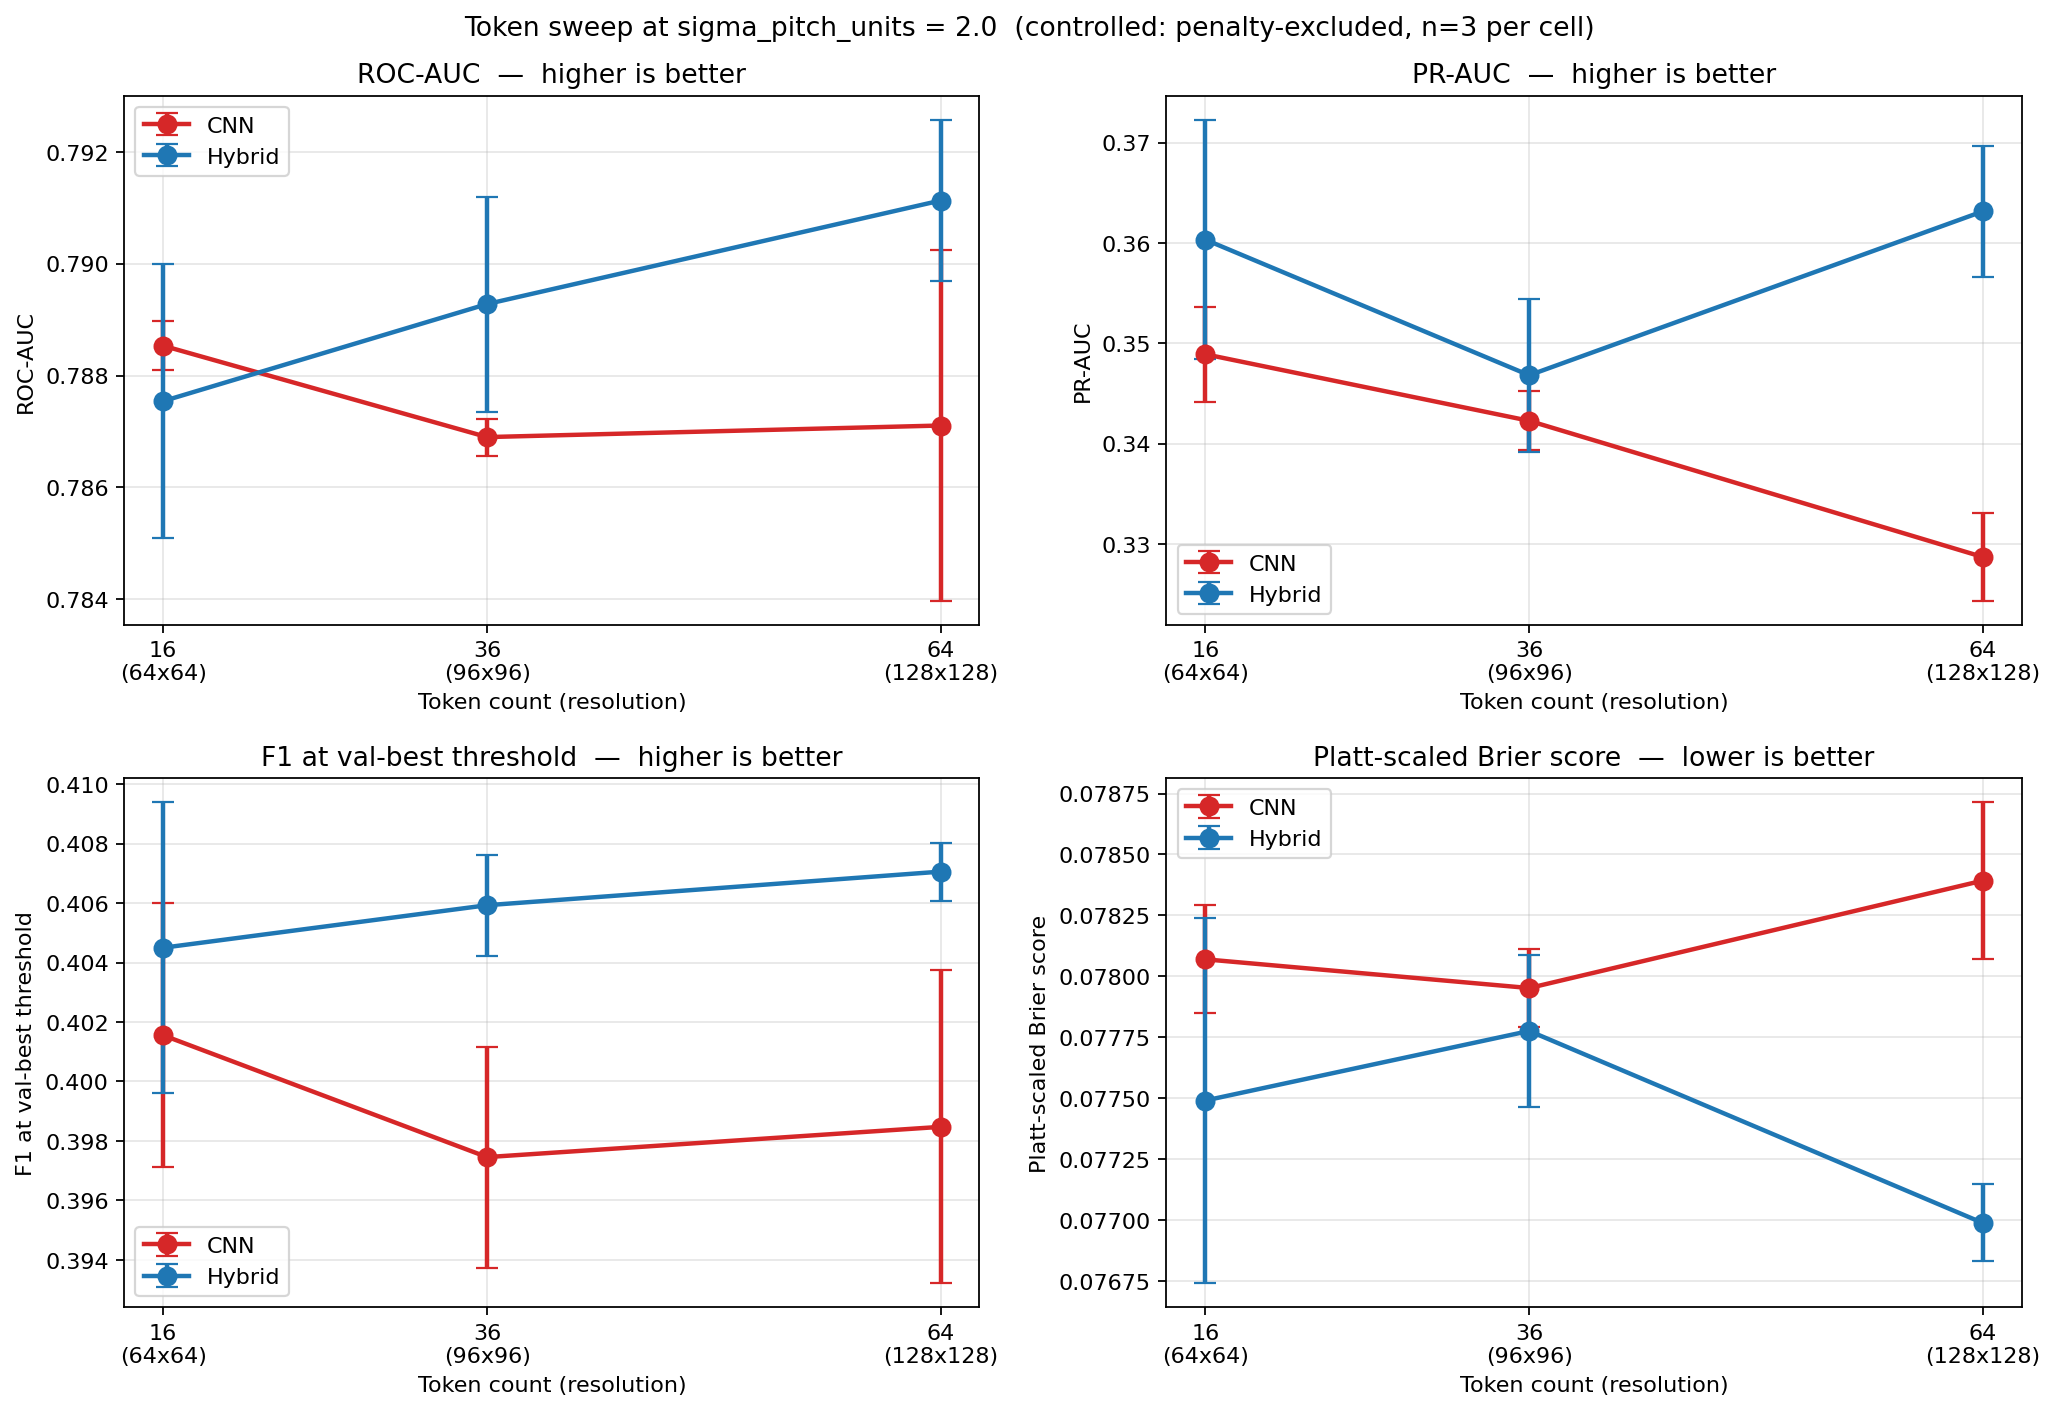
\includegraphics[width=0.92\linewidth]{figures/F1_token_sweep.png}
\caption{Token sweep at $\sigma_{\text{pu}}=2.0$ (controlled,
penalty-excluded, $n{=}3$ per cell). Hybrid lift over the same-resolution
CNN grows with token count on ROC-AUC, F1, and Brier; pure-CNN PR-AUC
degrades monotonically while the hybrid recovers at 64 tokens.}
\label{fig:token-sweep}
\end{figure}

\paragraph{Sigma Sweep at $128{\times}128$.}
\label{sec:sigma-sweep}
A single-seed sweep over
$\sigma_{\text{pu}} \in \{1.0, 2.0, 2.34, 3.5, 4.69\}$ at
$128{\times}128$ (full table in supplementary) places the test PR-AUC
peak at $\sigma_{\text{pu}}{=}2.0$ ($0.3337$); the pitch-equivalent of
the legacy 64-pixel baseline ($\sigma_{\text{pu}}{=}4.69$) is worse on
every metric ($0.3136$ PR-AUC, $0.0789$ Platt Brier). This is the
empirical motivation for specifying $\sigma$ in pitch-coordinate units:
pixel-fixed sigma scales the physical smoothing inversely with
resolution and is a hidden hyperparameter that materially affects
PR-AUC.

\subsection{Rendering Protocol Audit}
\label{sec:rendering-audit}

Before settling on the controlled rendering protocol, we audited three
candidate sources of cross-resolution inconsistency: the penalty
filter, sigma scaling with image resolution, and architecture
adaptation across resolutions. The audit identified $\sigma$ scaling
as the only material protocol mismatch: $\sigma$ had been fixed in
pixels, which silently halved the player blob's physical area when
resolution doubled, and this is what motivated the pitch-unit
specification in Section~\ref{sec:rendering}. The penalty filter and
the two architectures handled resolution changes correctly:
\texttt{AdaptiveAvgPool2d} in the CNN and a dynamically-sliced
positional embedding in the hybrid both adapt automatically to the
input size. The full audit log, including the visualization that motivated the $\sigma$ fix, is available in the release repository.

\subsection{$2{\times}2$ $\sigma\times$Penalty Ablation}
\label{sec:2x2}
% Source: EXPERIMENTS.md "Methodological note: 2x2 sigma x penalty ablation"

\begin{table}[t]
\centering
\caption{$2{\times}2$ $\sigma\times$penalty ablation at $64{\times}64$
($n{=}3$ per cell). \textbf{Penalty has near-zero main effect on PR-AUC;}
$\sigma$ has a positive average effect; the $\sigma\times$penalty
interaction is strong.}
\label{tab:2x2}
\resizebox{\textwidth}{!}{%
\begin{tabular}{lcccccc}
\toprule
Cell & $\sigma$ (pu) & Penalty & ROC-AUC & PR-AUC & F1 (val-best) & Platt Brier \\
\midrule
A & 2.0  & OUT & $0.7885\pm0.0004$ & $0.3489\pm0.0047$ & $0.4016\pm0.0044$ & $0.0781\pm0.0002$ \\
B & 2.0  & IN  & $0.7887\pm0.0002$ & $0.3397\pm0.0071$ & $0.3945\pm0.0054$ & $0.0791\pm0.0005$ \\
C & 4.69 & OUT & $0.7872\pm0.0017$ & $0.3533\pm0.0030$ & $0.3961\pm0.0065$ & $0.0775\pm0.0001$ \\
D & 4.69 & IN  & $0.7873\pm0.0021$ & $0.3624\pm0.0077$ & $0.3936\pm0.0032$ & $0.0780\pm0.0005$ \\
\midrule
\multicolumn{3}{l}{Penalty main effect} & $+0.0002$ & $-0.0001$ & $-0.0048$ & $+0.0008$ \\
\multicolumn{3}{l}{$\sigma$ main effect} & $-0.0014$ & $+0.0135$ & $-0.0031$ & $-0.0008$ \\
\multicolumn{3}{l}{Penalty $\times$ $\sigma$ interaction} & $\;\;0.0000$ & $\mathbf{+0.0183}$ & $+0.0045$ & $-0.0005$ \\
\bottomrule
\end{tabular}%
}
\end{table}

Comparing the controlled and legacy $64{\times}64$ runs changes
\emph{two} rendering variables simultaneously: $\sigma$ (pitch-unit
$\sigma_{\text{pu}}=2.0$ versus pixel-fixed $\sigma_{\text{px}}=2.5$,
i.e.\ $\sigma_{\text{pu}}\approx 4.69$ at $64{\times}64$) and penalty
handling (excluded versus included). To isolate the two effects we run
a $2{\times}2$ ablation (Table~\ref{tab:2x2}, three seeds per cell).

The penalty main effect on PR-AUC is $-0.0001$, essentially zero. The
$\sigma$ main effect on PR-AUC is $+0.0135$, and the $\sigma\times
\text{penalty}$ interaction is $+0.0183$. In particular, including
penalties helps PR-AUC at wide sigma (cell C $\rightarrow$ D:
$+0.0091$) but hurts at narrow sigma (cell A $\rightarrow$ B:
$-0.0092$): the penalty effect literally reverses sign with $\sigma$.
The cross-protocol A$\rightarrow$D PR-AUC gap of $+0.0135$ therefore
cannot be attributed to penalty inclusion alone; the correct
decomposition along the A$\rightarrow$C$\rightarrow$D path is
$+0.0044$ (the $\sigma$ change at penalty-out) plus $+0.0091$ (the
penalty change at wide $\sigma$). F1 (val-best) shows a cleaner
single-variable effect, a $-0.005$ penalty main effect, consistent
with the intuition that penalty inclusion shifts the
validation-selected threshold suboptimally. ROC-AUC and Brier are
essentially insensitive to either variable. The practical implication
for image-based xG protocols is that penalty handling and rendering
sigma do not compose linearly and should be reported together.

\subsection{Additional Analyses}
\label{sec:additional}

\textbf{Calibration.}
Figure~\ref{fig:calibration} shows reliability diagrams for four
representative cells from the six-cell headline (CNN/Hybrid at 64 and
128; the 96-cells, with Platt Brier $0.0780$ and $0.0778$ respectively,
sit between them). Raw probabilities are systematically over-confident
in the positive class because the \texttt{pos\_weight} of $\approx
8.85$ pushes the network toward high-probability outputs; raw Brier is
$\approx 0.20$ in every cell. A Platt calibrator~\cite{platt1999scaling}
fit on the validation predictions brings test Brier down to
$\approx 0.077$--$0.078$ in all six cells, with Hybrid 128 reaching the
lowest mean Platt Brier ($0.0770 \pm 0.0002$) and the tightest
standard-deviation band. Platt and isotonic
calibration~\cite{zadrozny2002transforming} give nearly identical Brier
on this dataset; we use Platt as the default since it preserves
ranking.

\begin{figure}[t]
\centering
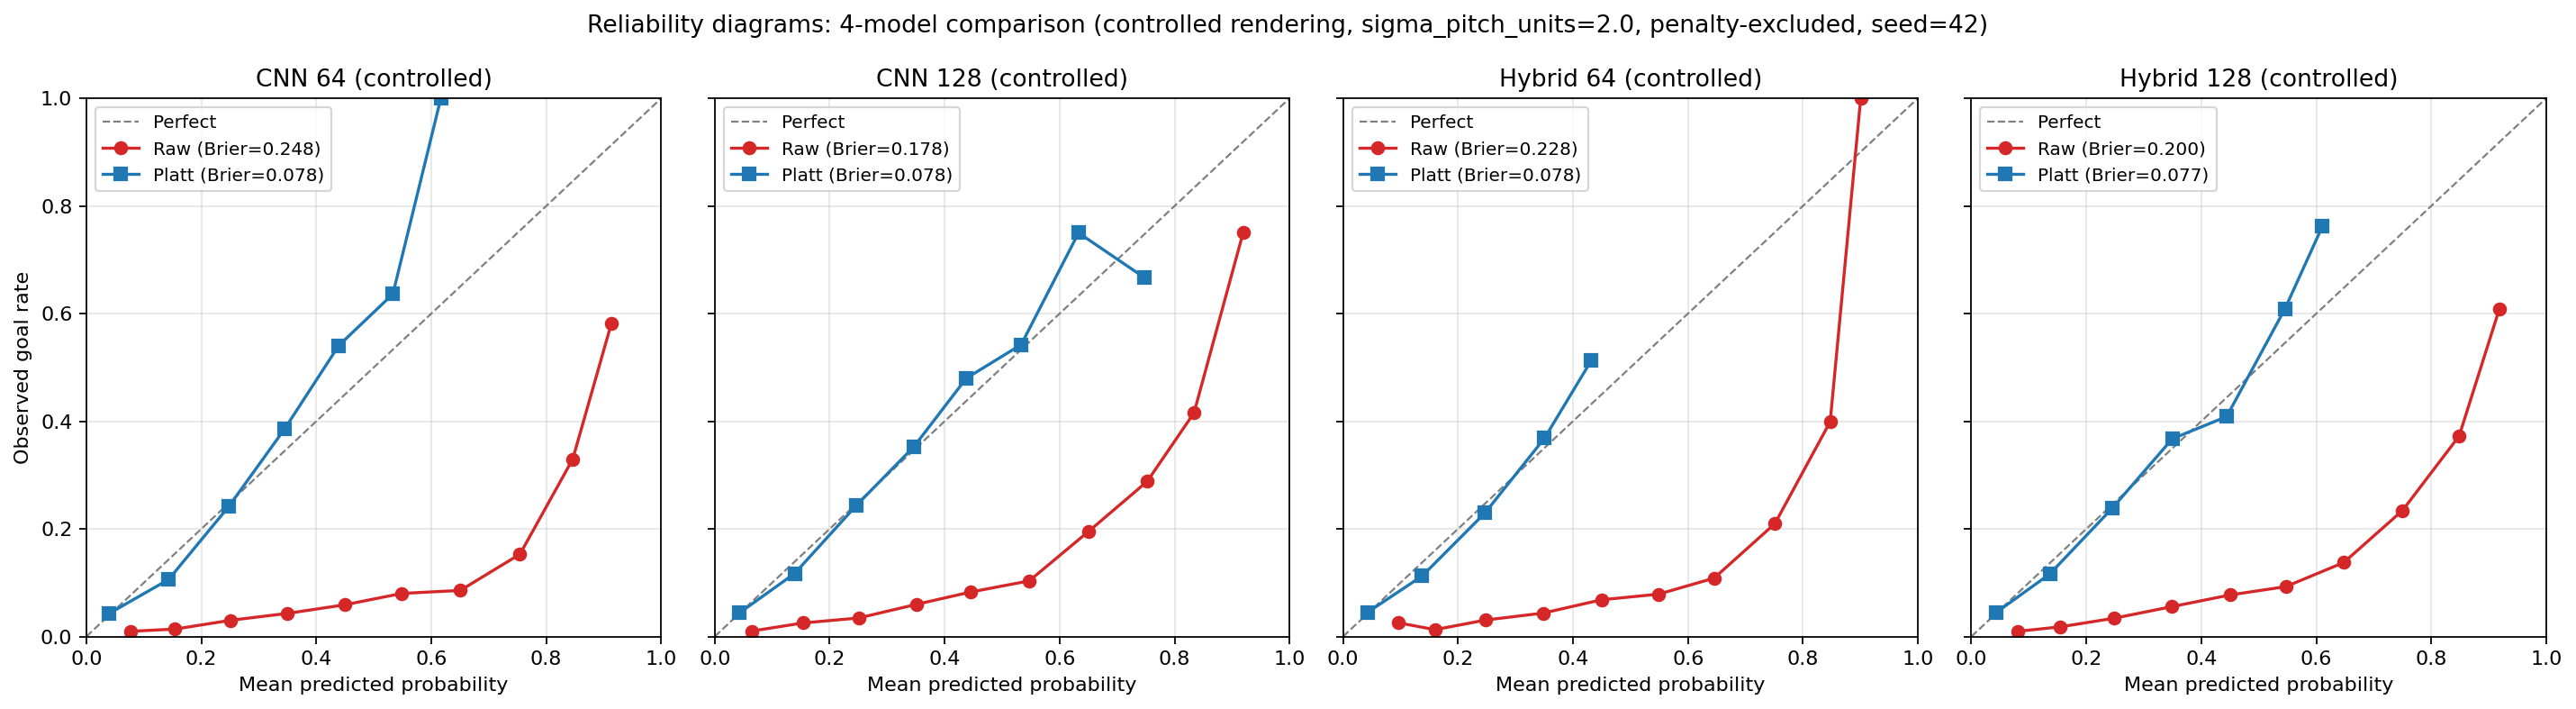
\includegraphics[width=\linewidth]{figures/F2_calibration.png}
\caption{Test-split reliability diagrams (10 bins) for four
representative cells from the six-cell headline (CNN/Hybrid at 64 and
128; controlled rendering, seed{=}42 checkpoint). Raw probabilities
are over-confident in the positive class because of
\texttt{pos\_weight}${=}8.85$; Platt scaling reduces test Brier to
$\approx 0.077$--$0.078$ in all four cells shown. Hybrid 128 has the
lowest Platt Brier across all six headline cells.}
\label{fig:calibration}
\end{figure}

\textbf{Attention rollout (qualitative).}
Attention rollout~\cite{abnar2020rollout} on Hybrid 128
$\sigma_{\text{pu}}{=}2.0$ (seed=42), visualized in the supplementary
material for four randomly selected goals from the test split,
concentrates on the goal-mouth area (the right side of the
attack-normalized pitch) and on defender and keeper clusters near the
shooter; midfield context receives essentially no attention. This is
consistent with how human analysts reason about xG (close-range
geometry around the box dominates the probability) and indicates that
the hybrid's transformer block is not exploiting spurious global
signals.

\textbf{Seed sensitivity.}
Across the six controlled headline cells, the seed standard deviation
ranges are ROC-AUC $0.0003$--$0.0031$, PR-AUC $0.0029$--$0.0119$,
F1 (val-best) $0.0010$--$0.0053$, and Platt Brier $0.0002$--$0.0007$.
PR-AUC seed std is therefore comparable in magnitude to typical
improvements claimed in image-based xG comparisons; we recommend a
three-seed minimum for any such comparison. A five-seed sensitivity on
a legacy mixed-protocol pair is available in the release repository.

\section{Discussion}
\label{sec:discussion}

Three observations stand out. First, the hybrid's value here is
conditional on token count: at 16 tokens it is essentially tied with
the CNN, while at 64 tokens it improves every headline metric. Second,
the pure CNN under-uses higher resolution under controlled rendering;
PR-AUC degrades monotonically as resolution grows
(Section~\ref{sec:headline}). The conv-pool-then-global-pool design
discards the additional spatial detail at the AdaptiveAvgPool, whereas
the transformer block turns that detail into a measurable
improvement. Third, two rendering choices that are often hidden in
implementation details, the Gaussian sigma and the penalty filter, do
not compose linearly: under our $2{\times}2$ ablation the penalty main
effect on PR-AUC is essentially zero while the
$\sigma\times\text{penalty}$ interaction is large, so the apparent
penalty bias observed in any single cross-protocol comparison is
itself a function of $\sigma$. Specifying $\sigma$ in pitch-coordinate
units rather than pixels removes one of the two hidden variables.

\section{Limitations}
\label{sec:limitations}

We use a single open dataset; cross-dataset generalization is not
tested. Penalty exclusion is necessary for renderable consistency but
removes a small amount of structurally distinct shot context. At
$64{\times}64$ the controlled $\sigma_{\text{pu}}=2.0$ corresponds to
$\sigma_{\text{px}}\approx 1.07$, sharp enough that the model overfits
quickly (best validation epoch at 3--6); a separate $64{\times}64$
$\sigma$ sweep is future work. We report seed variability for every
controlled cell, but we did not separately isolate hardware or backend
nondeterminism on the MPS device; both effects are mixed into the
reported standard deviations. The numeric comparison to xG-CNN is
indirect (different channel structure, pitch
coverage, grid, dataset filter, and validation protocol); we treat
xG-CNN as methodological motivation rather than a baseline, and a
strict replication under our protocol is future work.

\section{Conclusion and Future Work}
\label{sec:conclusion}

Under a strictly controlled rendering protocol, a CNN+Transformer
hybrid at $128{\times}128$ outperforms a $64{\times}64$ CNN baseline
on every headline metric for image-based Expected Goals. The lift is
conditional on transformer token count, and the central observation
is that pure CNN PR-AUC degrades monotonically with input resolution
while the hybrid recovers at 64 tokens. We argue that the rendering
sigma is a hidden hyperparameter that should be specified in
pitch-coordinate units, and we show via a $2{\times}2$ ablation that
penalty inclusion has no single-variable PR-AUC effect; its impact is
$\sigma$-conditional. Future work includes a $\sigma$ sweep at
$64{\times}64$ and $96{\times}96$, a ViT-XG variant at $128{\times}128$
that the code base supports but we have not trained, and a strict
xG-CNN replication under our protocol.

% ============================================================
% Acknowledgements (optional, after notification)
% ============================================================
\subsubsection*{Reproducibility.}
The release repository is available at
\url{https://github.com/mburkay/image-xg-cnn-transformer}. It contains the source code, splits,
the paper \LaTeX{} source, and the supplementary documentation: the
full hyperparameter table, the five-seed sensitivity on the legacy
mixed-protocol pair, the $2{\times}2$ ablation derivation, and the
rendering-protocol audit log. The 38 model checkpoints
(${\approx}\,600$\,MB) and the rendered image datasets will be
deposited on a public archive (Zenodo or equivalent) upon
acceptance, with the DOI added to the repository README.

% ============================================================
% REFERENCES (unlimited length per MLSA 2026 CFP)
% ============================================================
\bibliographystyle{splncs04}
\bibliography{references}

\end{document}
